\documentclass[aos,preprint]{imsart}

%\usepackage{amsthm,amsmath,natbib}
%\RequirePackage[colorlinks,citecolor=blue,urlcolor=blue]{hyperref}

% provide arXiv number if available:
%\arxiv{arXiv:0000.0000}

% put your definitions there:
\usepackage[autonum]{macros}
\usepackage{natbib}

\allowdisplaybreaks

\begin{document}

\begin{frontmatter}
\title{A zero-inflated analysis of the 2020 Tour de France}
%\title{A sample article title with some additional note\thanksref{t1}}
\runtitle{A zero-inflated analysis of the 2020 Tour de France}
%\thankstext{T1}{A sample additional note to the title.}

\begin{aug}
\author{\fnms{Gian Carlo} \snm{Di-Luvi}\thanksref{m1}},

\runauthor{}

\affiliation{University of British Columbia\thanksmark{m1}}

\address{Department of Statistics\\
University of British Columbia\\
Vancouver, BC, Canada V6T 1Z4\\
E-mail: \normalfont
\href{mailto:gian.diluvi@stat.ubc.ca}{gian.diluvi@stat.ubc.ca},}

\end{aug}

\begin{abstract}
Lorem ipsum dolor sit amet, consectetur adipisicing elit, sed do eiusmod tempor incididunt ut labore et dolore magna aliqua. Ut enim ad minim veniam, quis nostrud exercitation ullamco laboris nisi ut aliquip ex ea commodo consequat. Duis aute irure dolor in reprehenderit in voluptate velit esse cillum dolore eu fugiat nulla pariatur. Excepteur sint occaecat cupidatat non proident, sunt in culpa qui officia deserunt mollit anim id est laborum.
\end{abstract}

%\begin{keyword}
%\kwd{a keyword}
%\end{keyword}

\end{frontmatter}

\section{Introduction} \label{sec:intro}


\section{Data description} \label{sec:data}


The data contain information of each cyclist and stage of the 2020 Tour de France. A summary of all the variables included in the data set can be found in Table \ref{table:data}. The data are public and was scraped from the \href{letour.fr}{Tour's official website} using \texttt{Python} and the \href{https://en.wikipedia.org/wiki/2020_Tour_de_France}{2020 Tour de France Wikipedia} page by hand. It was then combined into a single data set containing 3,390 observations and 23 variables. \\

Each row corresponds to an observation and each column to a variable. The observations are at the ``rider by stage'' level, i.e., each observation corresponds to a rider at a given stage. Some variables, such as the winner country, are constant across stages. The number of riders is not the same at each stage because some riders leave the race due to injuries. Specifically, 175 riders started the tour but only 146 finished it.\footnote{Notably, Egan Bernal, last year's winner, left the Tour after stage 16 due to back pain.} There are five different stage types in this data set: flat, medium mountain, hilly, mountain, and mountain time trial. Other stage types exist in the sport but were not included in this year's Tour de France (e.g. team time trial). The cumulative time is determined as the sum of the times at each stage, minus the total bonus seconds, plus the total penalty seconds. Bonus points are awarded to the first three riders to finish each stage; penalties are impossed when cyclists break rules, such as receiving food close to the finish line. Finally, race leader is used interchangeably with general classification leader because that is the most important event of the Tour, even though there are many races going on at the same time.



\begin{table}[ht]
\centering
\begin{tabular}{lll}
\textbf{Variable} & \textbf{Description}                                                                                                  & \textbf{Type of variable} \\ \hline
rank              & rider's rank at that stage                                                                                            & float                     \\
rider             & rider's name                                                                                                          & string                    \\
rider\_number     & rider's bib number                                                                                                    & integer                   \\
team              & rider's team                                                                                                          & string                    \\
time              & rider's time in that stage                                                                                            & string                    \\
bonus             & rider's bonus seconds in that stage                                                                                   & float                     \\
penalty           & rider's penalty seconds in that stage                                                                                 & float                     \\
stage             & stage number                                                                                                          & integer                   \\
date              & date of stage                                                                                                         & date                      \\
distance          & distance of stage                                                                                                     & float                     \\
origin            & origin of stage                                                                                                       & string                    \\
destination       & destination of stage                                                                                                  & string                    \\
stage\_type       & type of stage (mountain, flat, etc.)                                                                                  & string                    \\
winner\_country   & country of rider who won stage                                                                                        & string                    \\
general           & bib number of rider leading the race                                                                                  & integer                   \\
points            & bib number of rider leading the points race                                                                           & integer                   \\
mountains         & bib number of rider leading the mountains race                                                                        & integer                   \\
young             & bib number of rider leading the young race                                                                            & integer                   \\
stage\_winner     & bib number of rider that won the stage                                                                                & integer                   \\
time\_seconds     & rider's time in seconds in that stage                                                                                 & float                     \\
cum\_time         & \begin{tabular}[c]{@{}l@{}}rider's cumulative time at that stage\\ (including bonus and penalty seconds)\end{tabular} & float                     \\
gc\_rank          & rider's rank in the general classification                                                                            & integer                   \\
timediff          & rider's time difference in seconds to race leader                                                                     & float                     \\ \hline
\end{tabular}
\caption{Variables included in the data set.}
\label{table:data}
\end{table}



\section{Exploratory data analysis} \label{sec:eda}


Stage number plays an important role because, as the race progresses, the riders become more tired. There were two rest days between stages 9 and 10 and 15 and 16. Tour de France riders can recover at faster rates than average people, so that their performance after a rest day could be similar to their performance during the Tour's first stage. In any case, performance can vary significantly by stage.

To address the statistical question, we could directly work with the rank at each stage. However, as we will argue in Section \ref{sec:stats}, working with this variable leads to many statistical complications. We instead explore variables that are not exactly the rank, but that can be used to determine it and are more amenable to statistical modelling. Figure \ref{fig:cumtime} shows the cumulative time of riders by stage. Cumlative time seems to increase linearly by stage, which suggests that a linear regression model might be appropriate. There are, however, some issues with this variable. First, the variance of the observations increases with stage. This is due to the fact that cumulative time is determined by adding individual stage times. The more times are added, the more variability there will be. Second, the observations are not independent: clearly a rider's cumulative time has to increase from one stage to the next. This also imposes a non-trivial combinatorial constraint that makes working with cumulative time too complicated. \\


\begin{figure}[h]
  \centering
  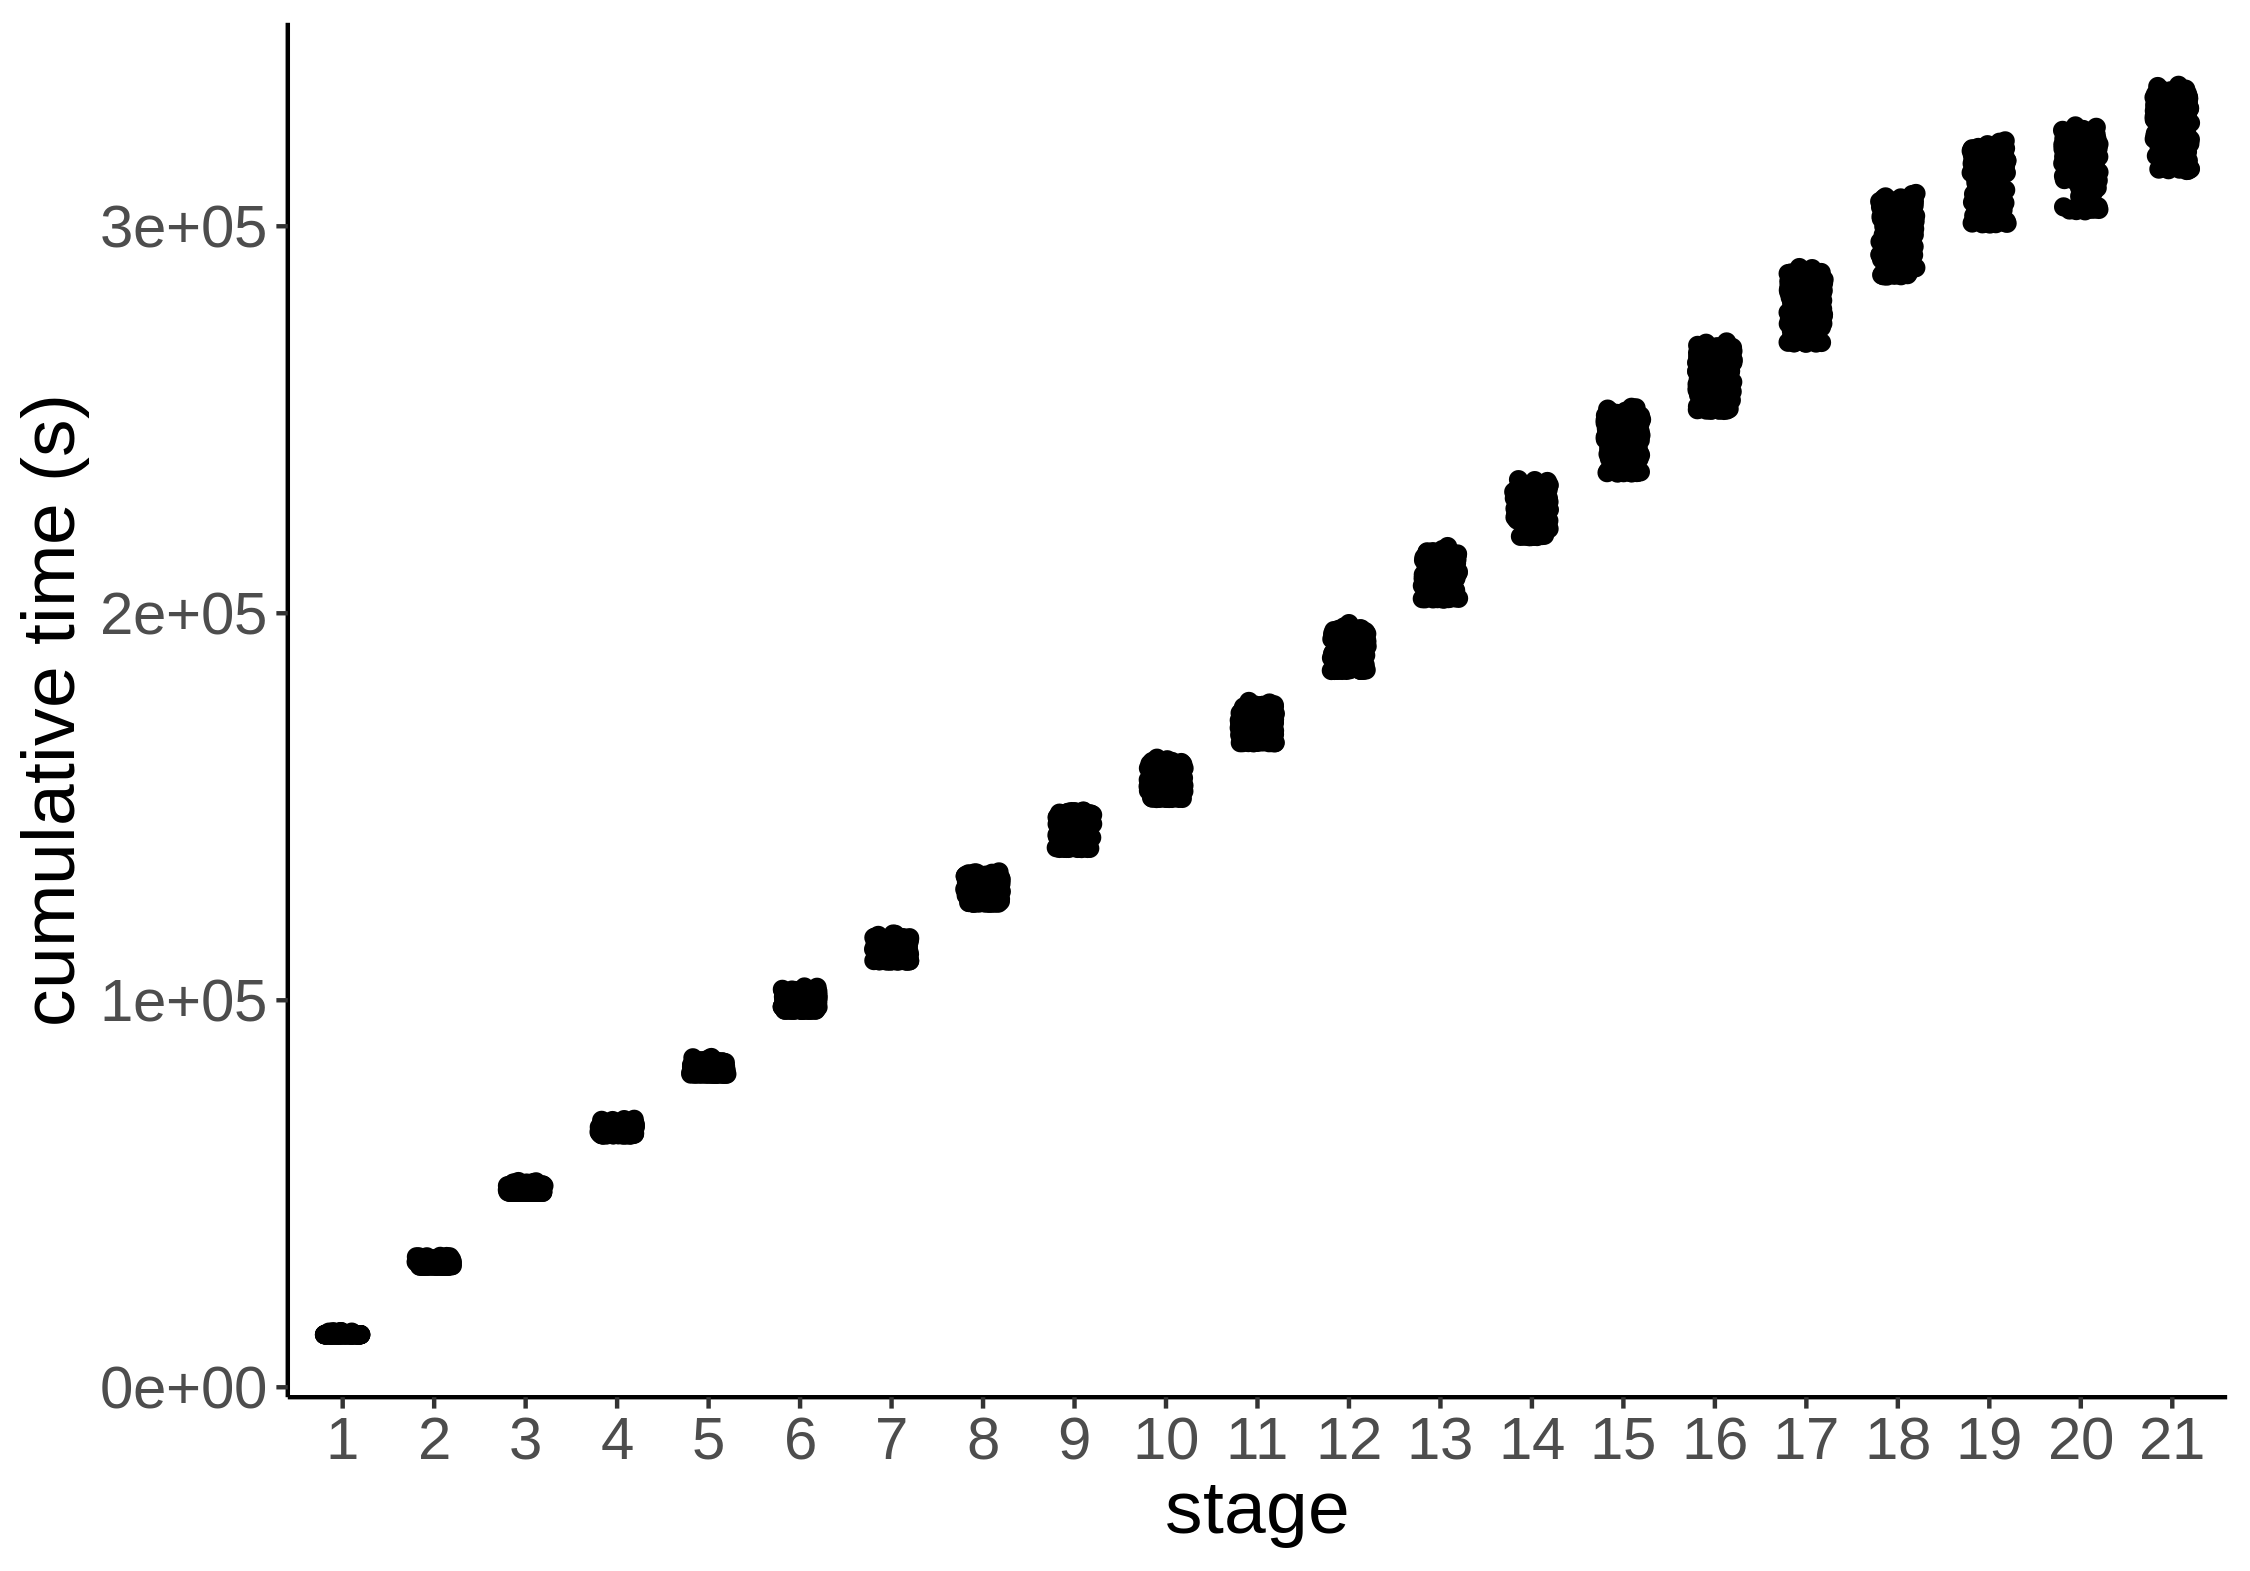
\includegraphics[scale=0.65]{fig/cumtime_stage.png}
  \caption{Scatterplot of cumulative time by stage. Each point corresponds to a rider's cumulative time at the corresponding stage.}
  \label{fig:cumtime}
\end{figure}


One alternative to cumulative time is the time difference of every rider to the race leader at every stage. A visual inspection of Figure \ref{fig:timediff_stage}, which shows how time differences vary through stage, suggests a linear relationship between stage and time difference. As was the case of cumulative time, the variance of the time difference also increases with stage---for similar reasons as before. Although time difference also resulst in a combinatorially complicated structure, it is not nearly as complicated as the one induced by the cumulative time. The model proposed in Section \ref{sec:stats} addresses these issues. \\



\begin{figure}[h]
  \centering
  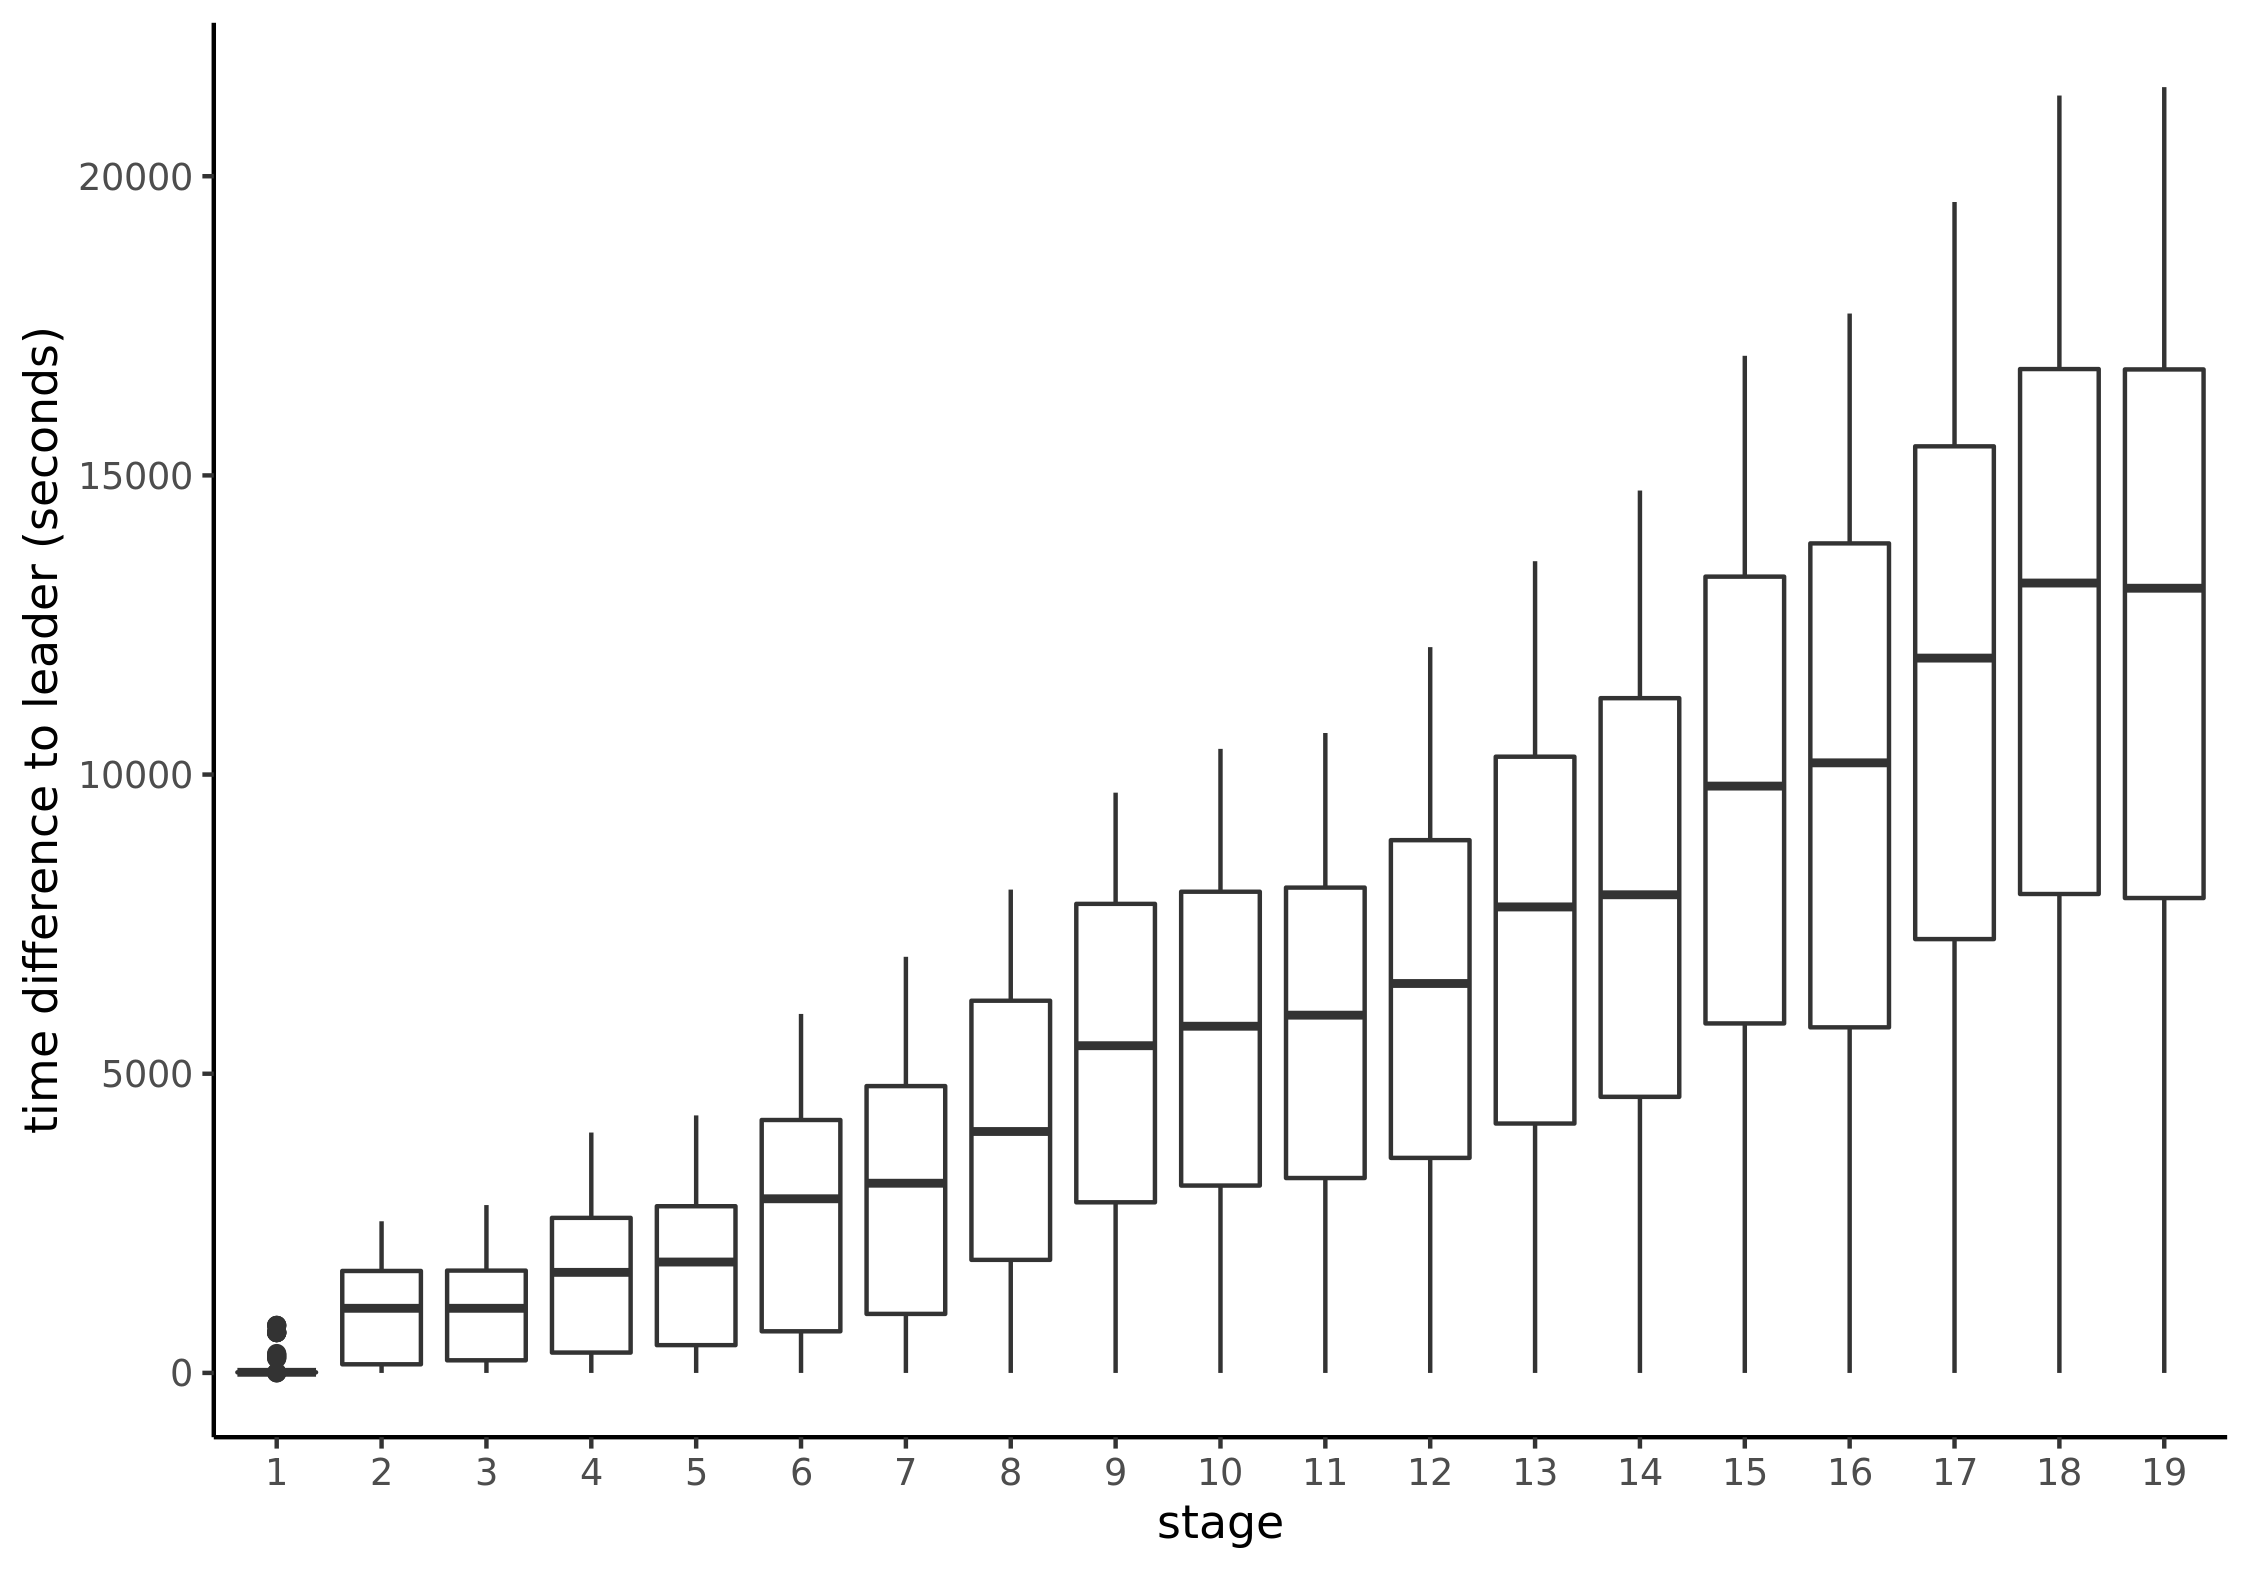
\includegraphics[scale=0.65]{fig/timediff_stage.png}
  \caption{Boxplots of time difference to leader for every stage. The variability in the time difference increases as stages progress.}
  \label{fig:timediff_stage}
\end{figure}



%\begin{figure}[h]
%  \centering
%  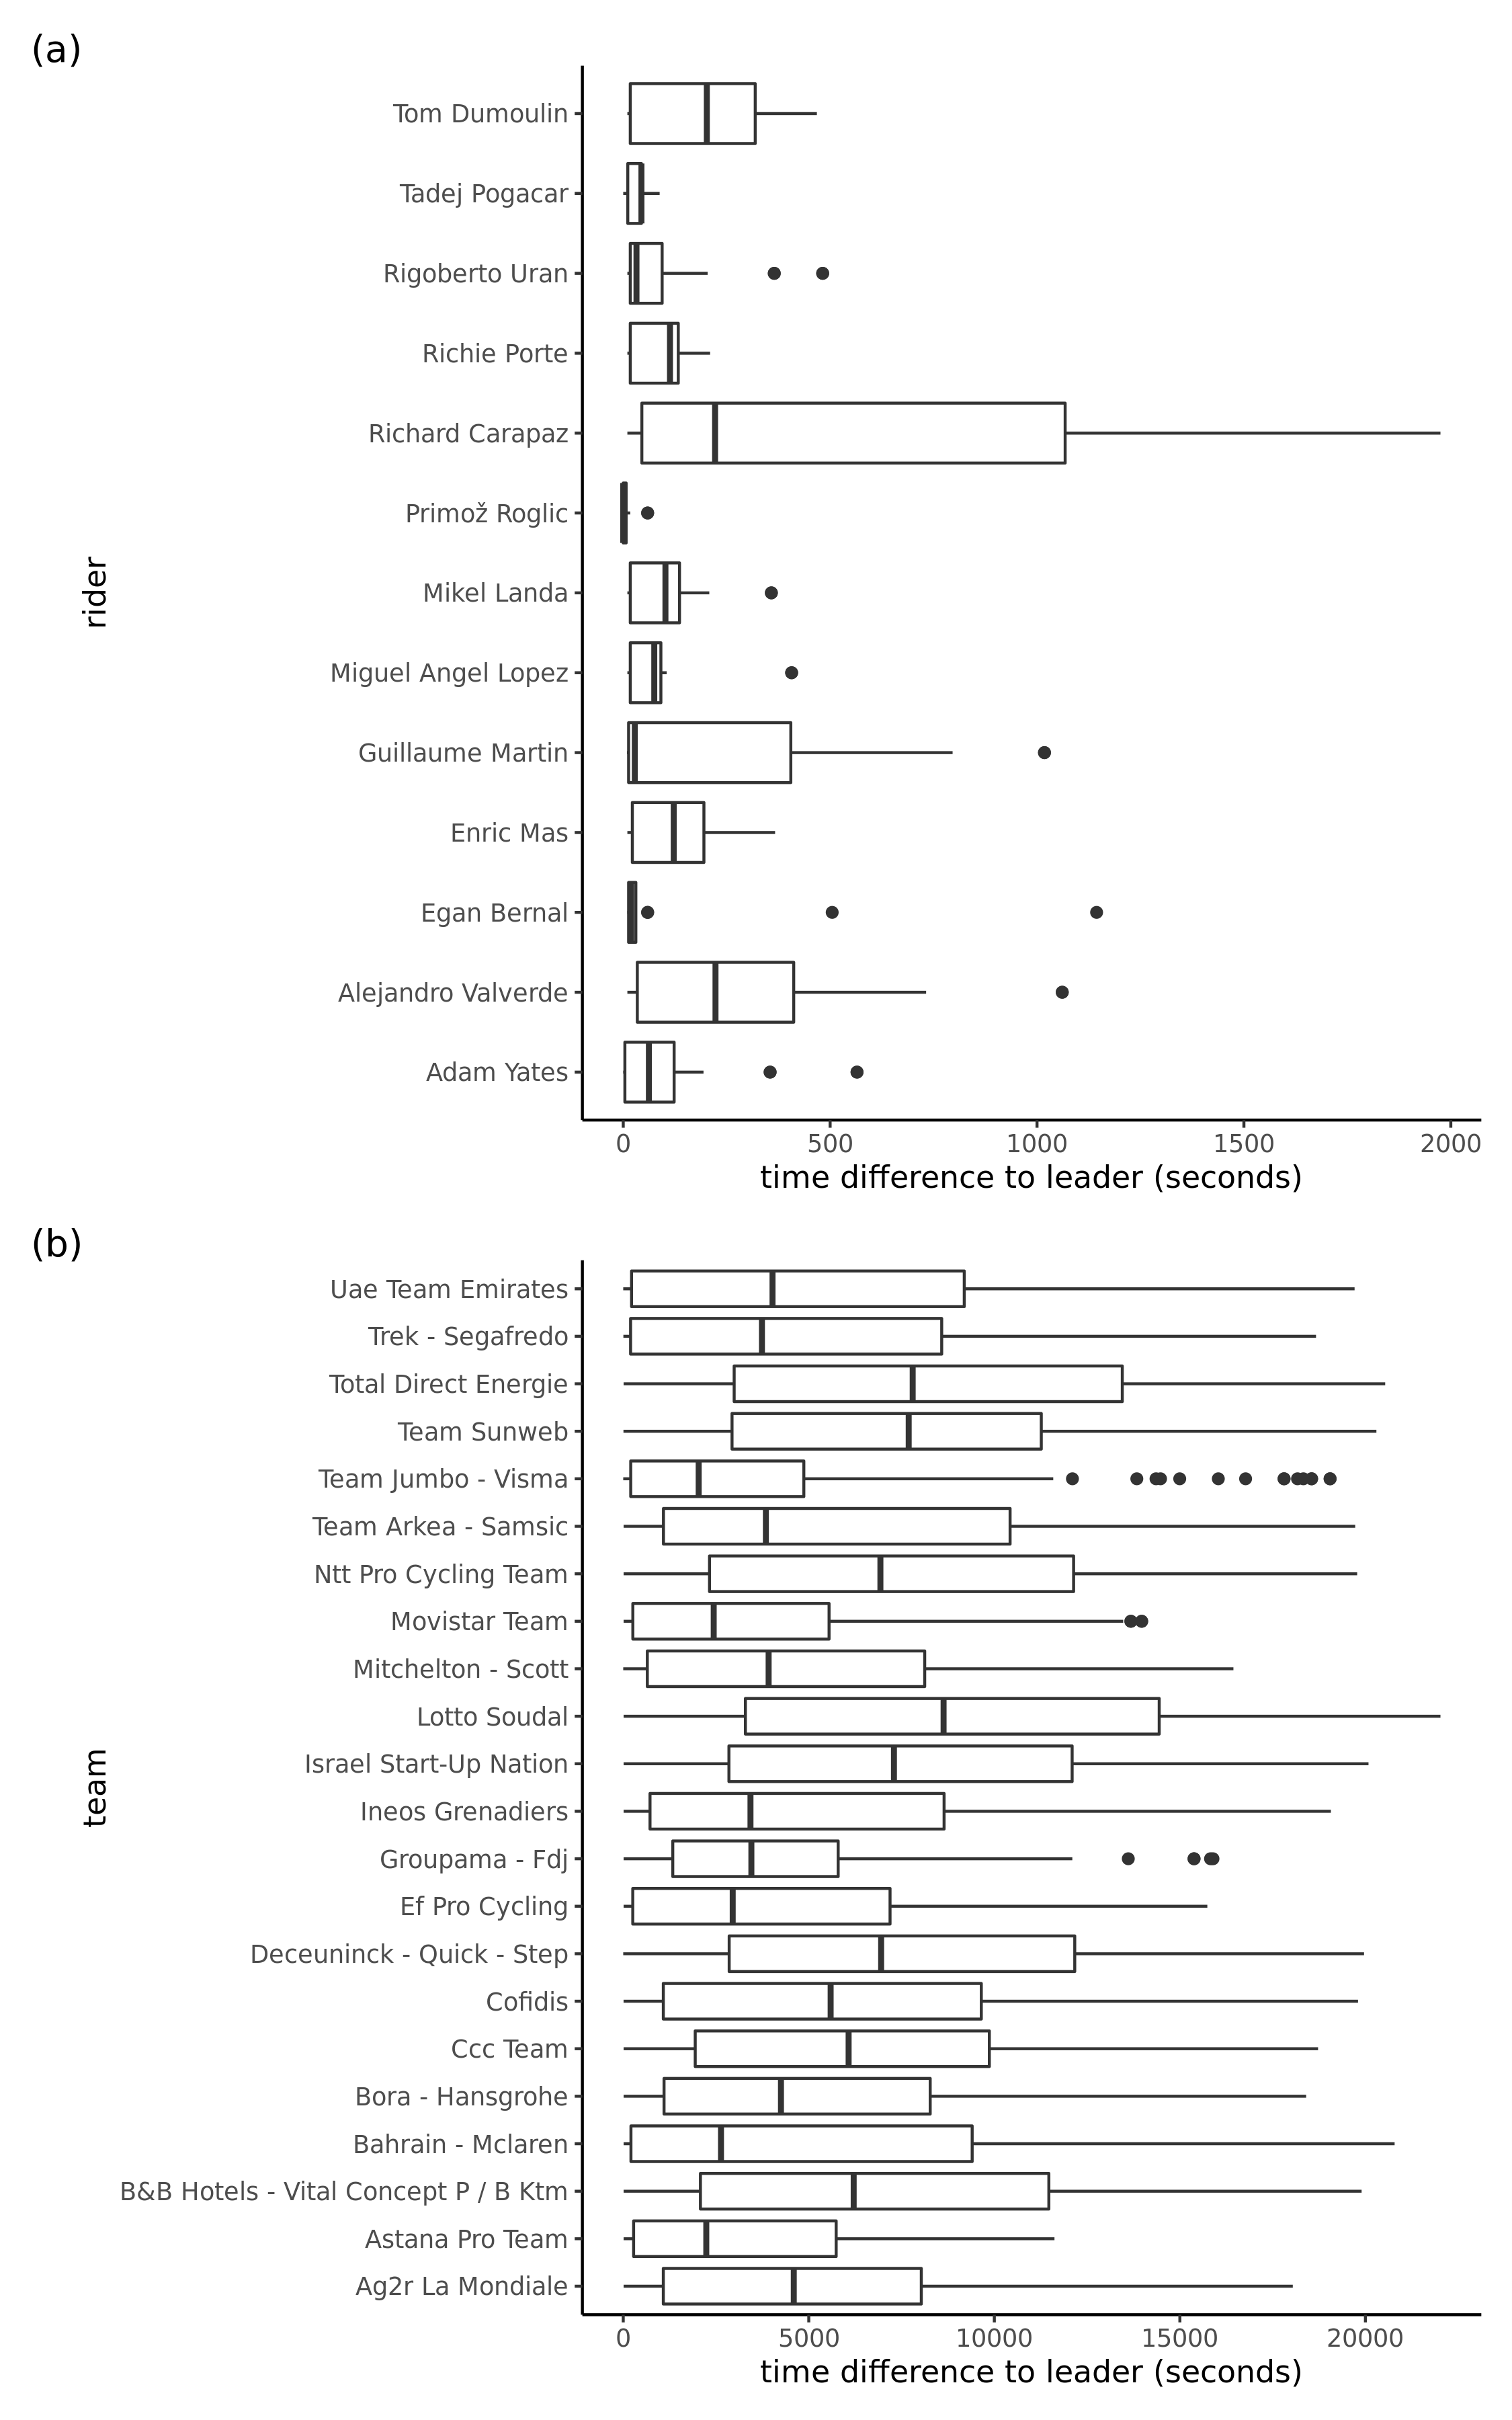
\includegraphics[scale=0.4]{fig/timediff_contender_team.png}
%  \caption{Boxplots of time difference to leader for every top contender and team. Contenders seem to vary more between them than teams.}
%  \label{fig:timediff_contender_team}
%\end{figure}


\begin{figure}[h]
  \centering
  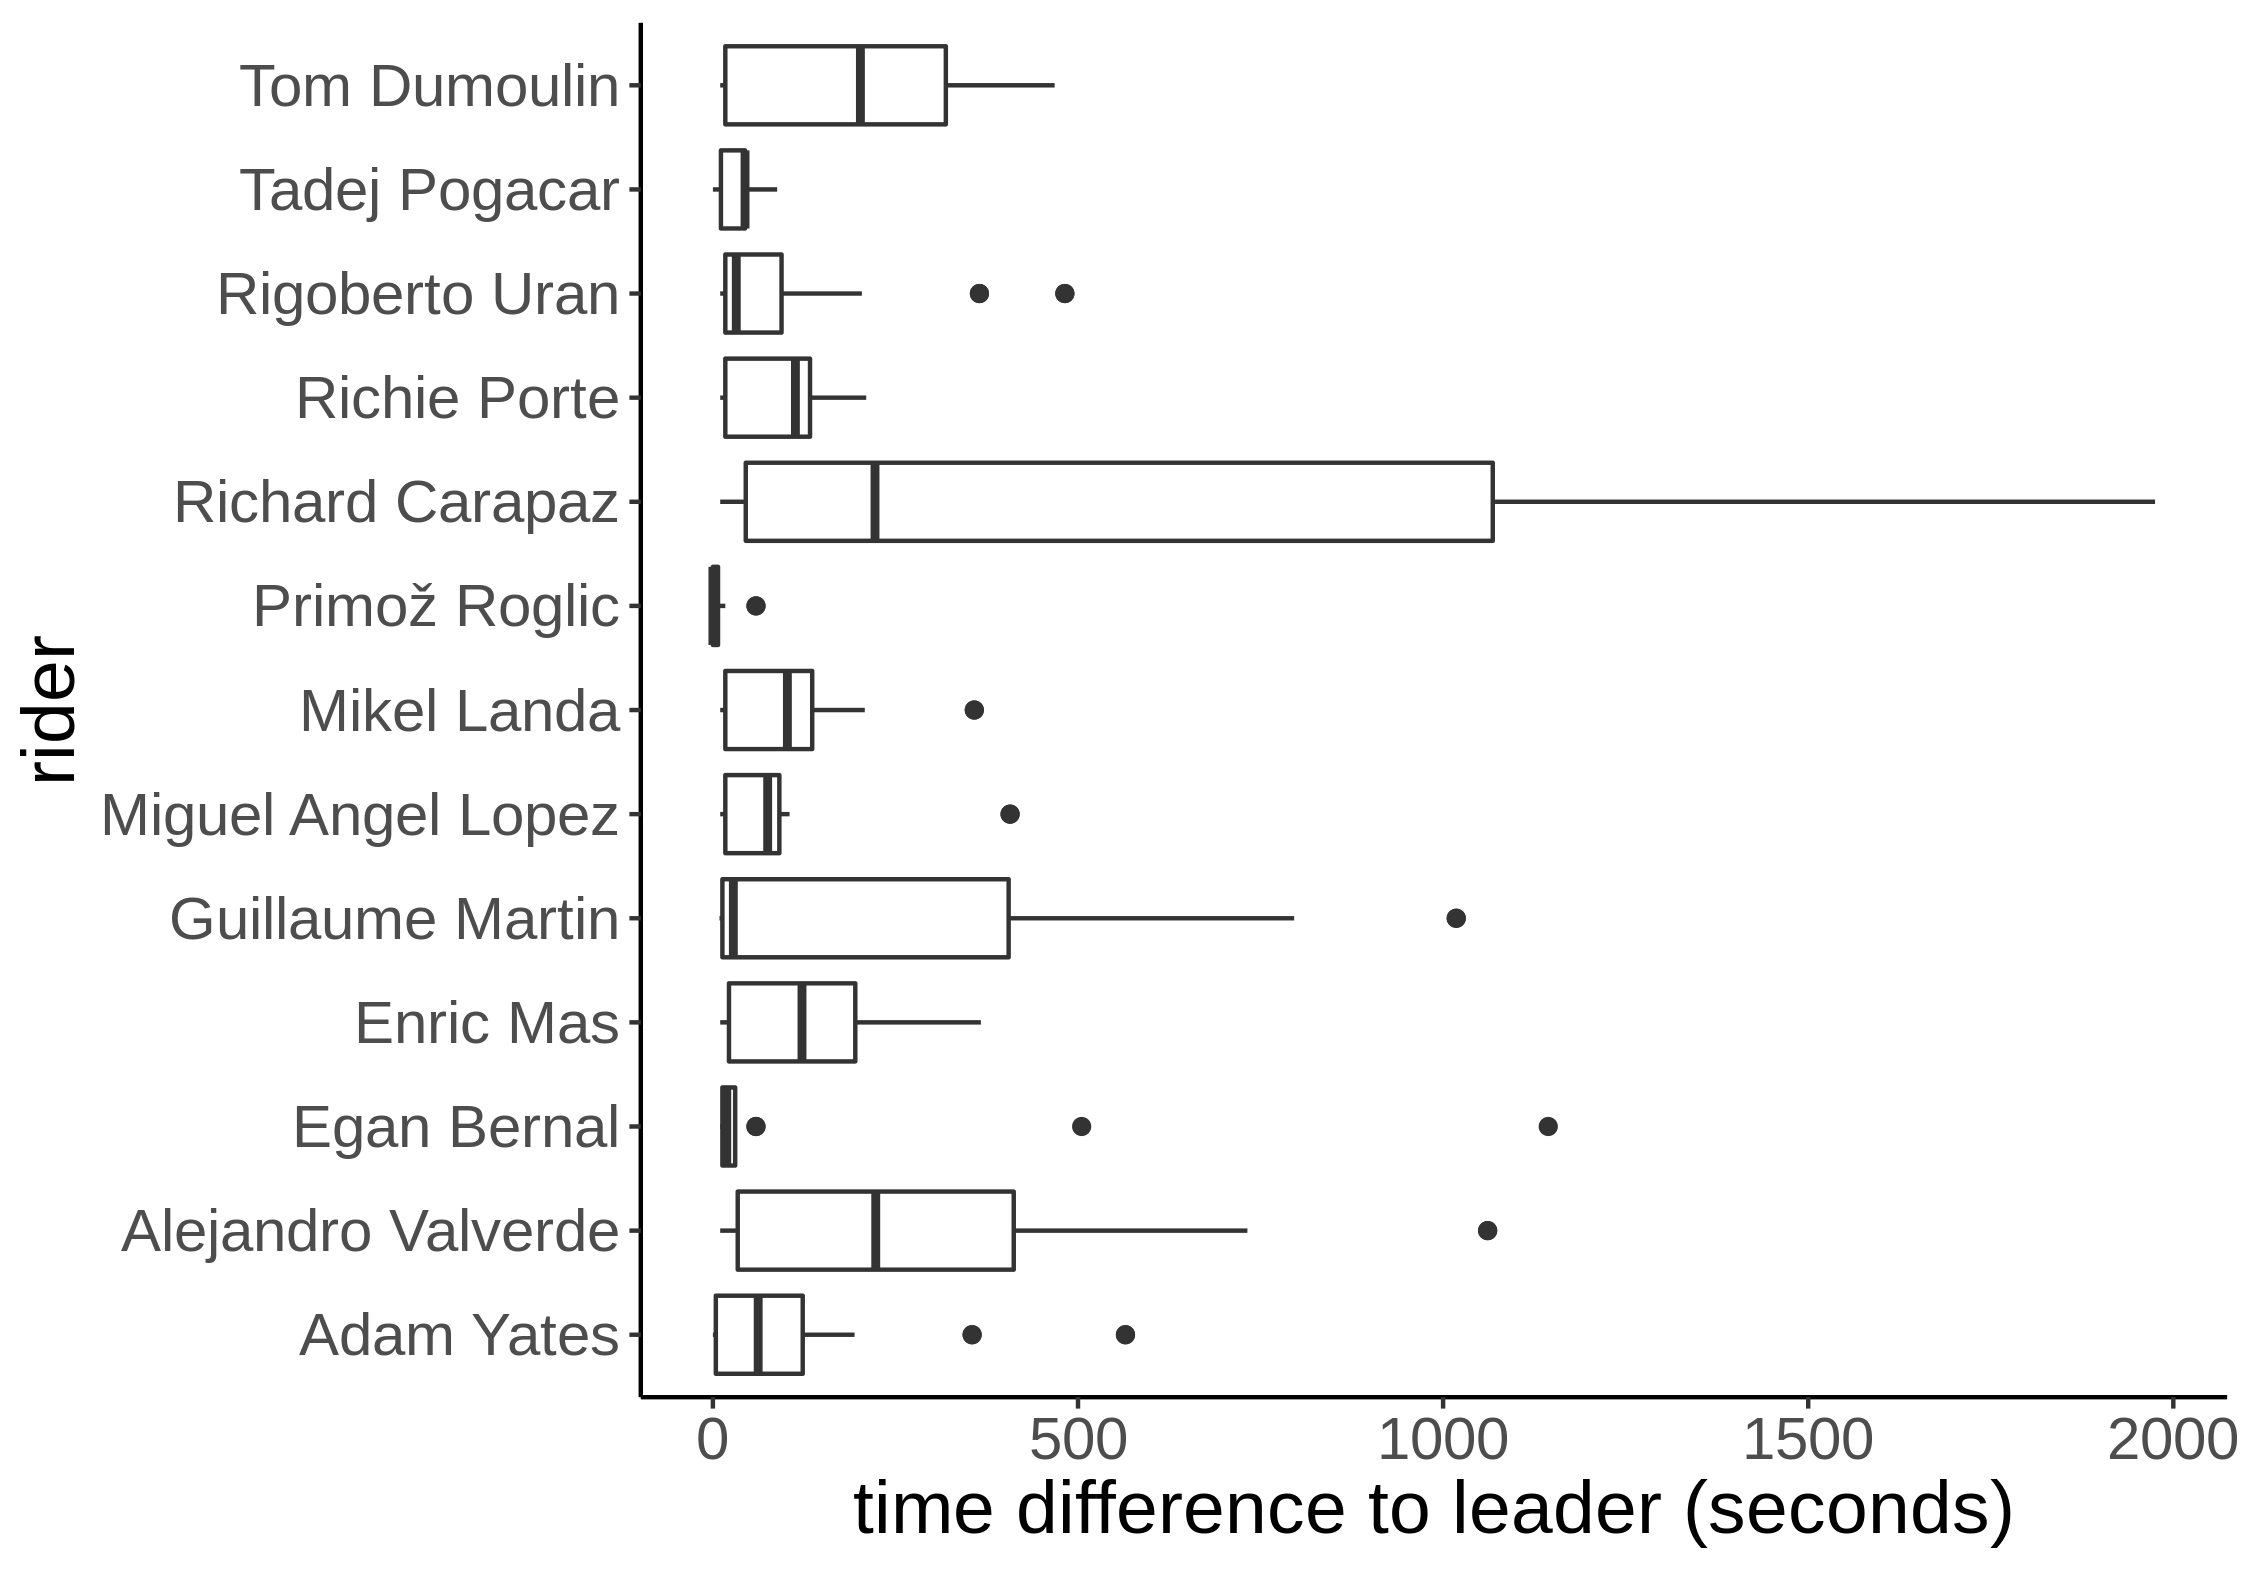
\includegraphics[scale=0.65]{fig/timediff_contender.png}
  \caption{Boxplots of time difference to leader for every top contender. Contenders seem to vary between them, even if they were all contesting the Tour.}
  \label{fig:timediff_contender}
\end{figure}


\begin{figure}[h]
  \centering
  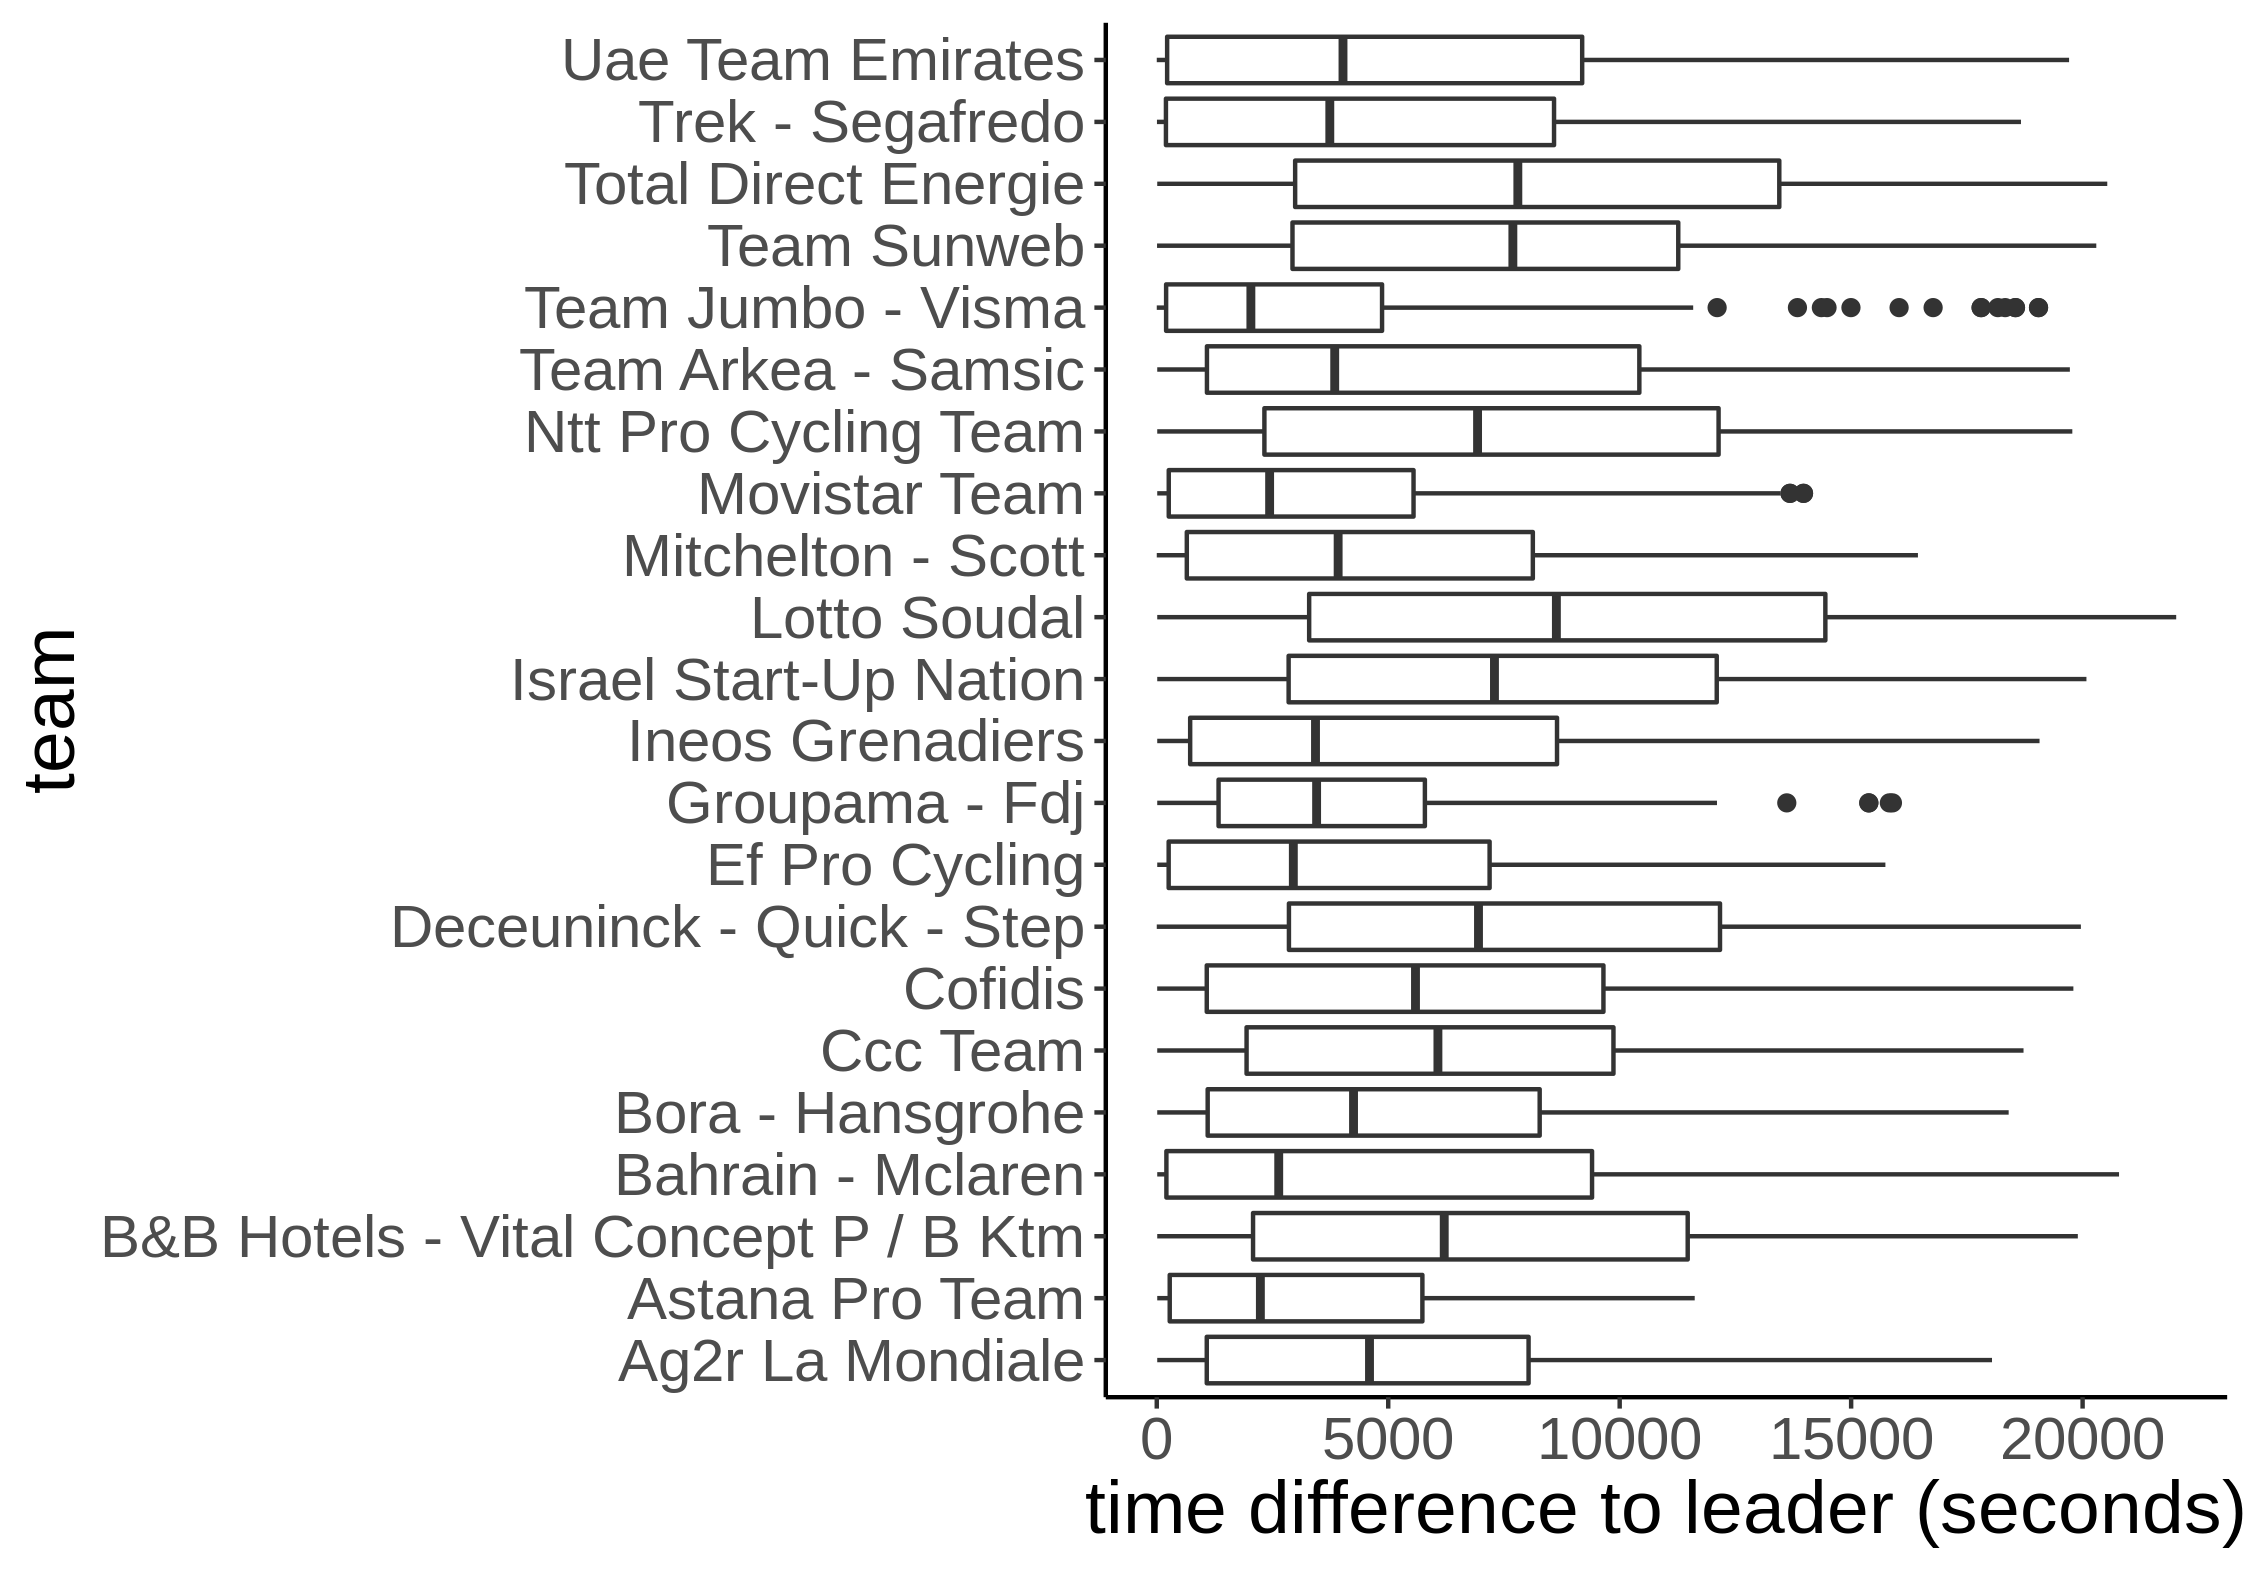
\includegraphics[scale=0.65]{fig/timediff_team.png}
  \caption{Boxplots of time difference to leader for every team. Contenders seem to vary more between them than teams.}
  \label{fig:timediff_team}
\end{figure}






\section{Statistical methodologies} \label{sec:stats}



\begin{figure}[h]
  \centering
  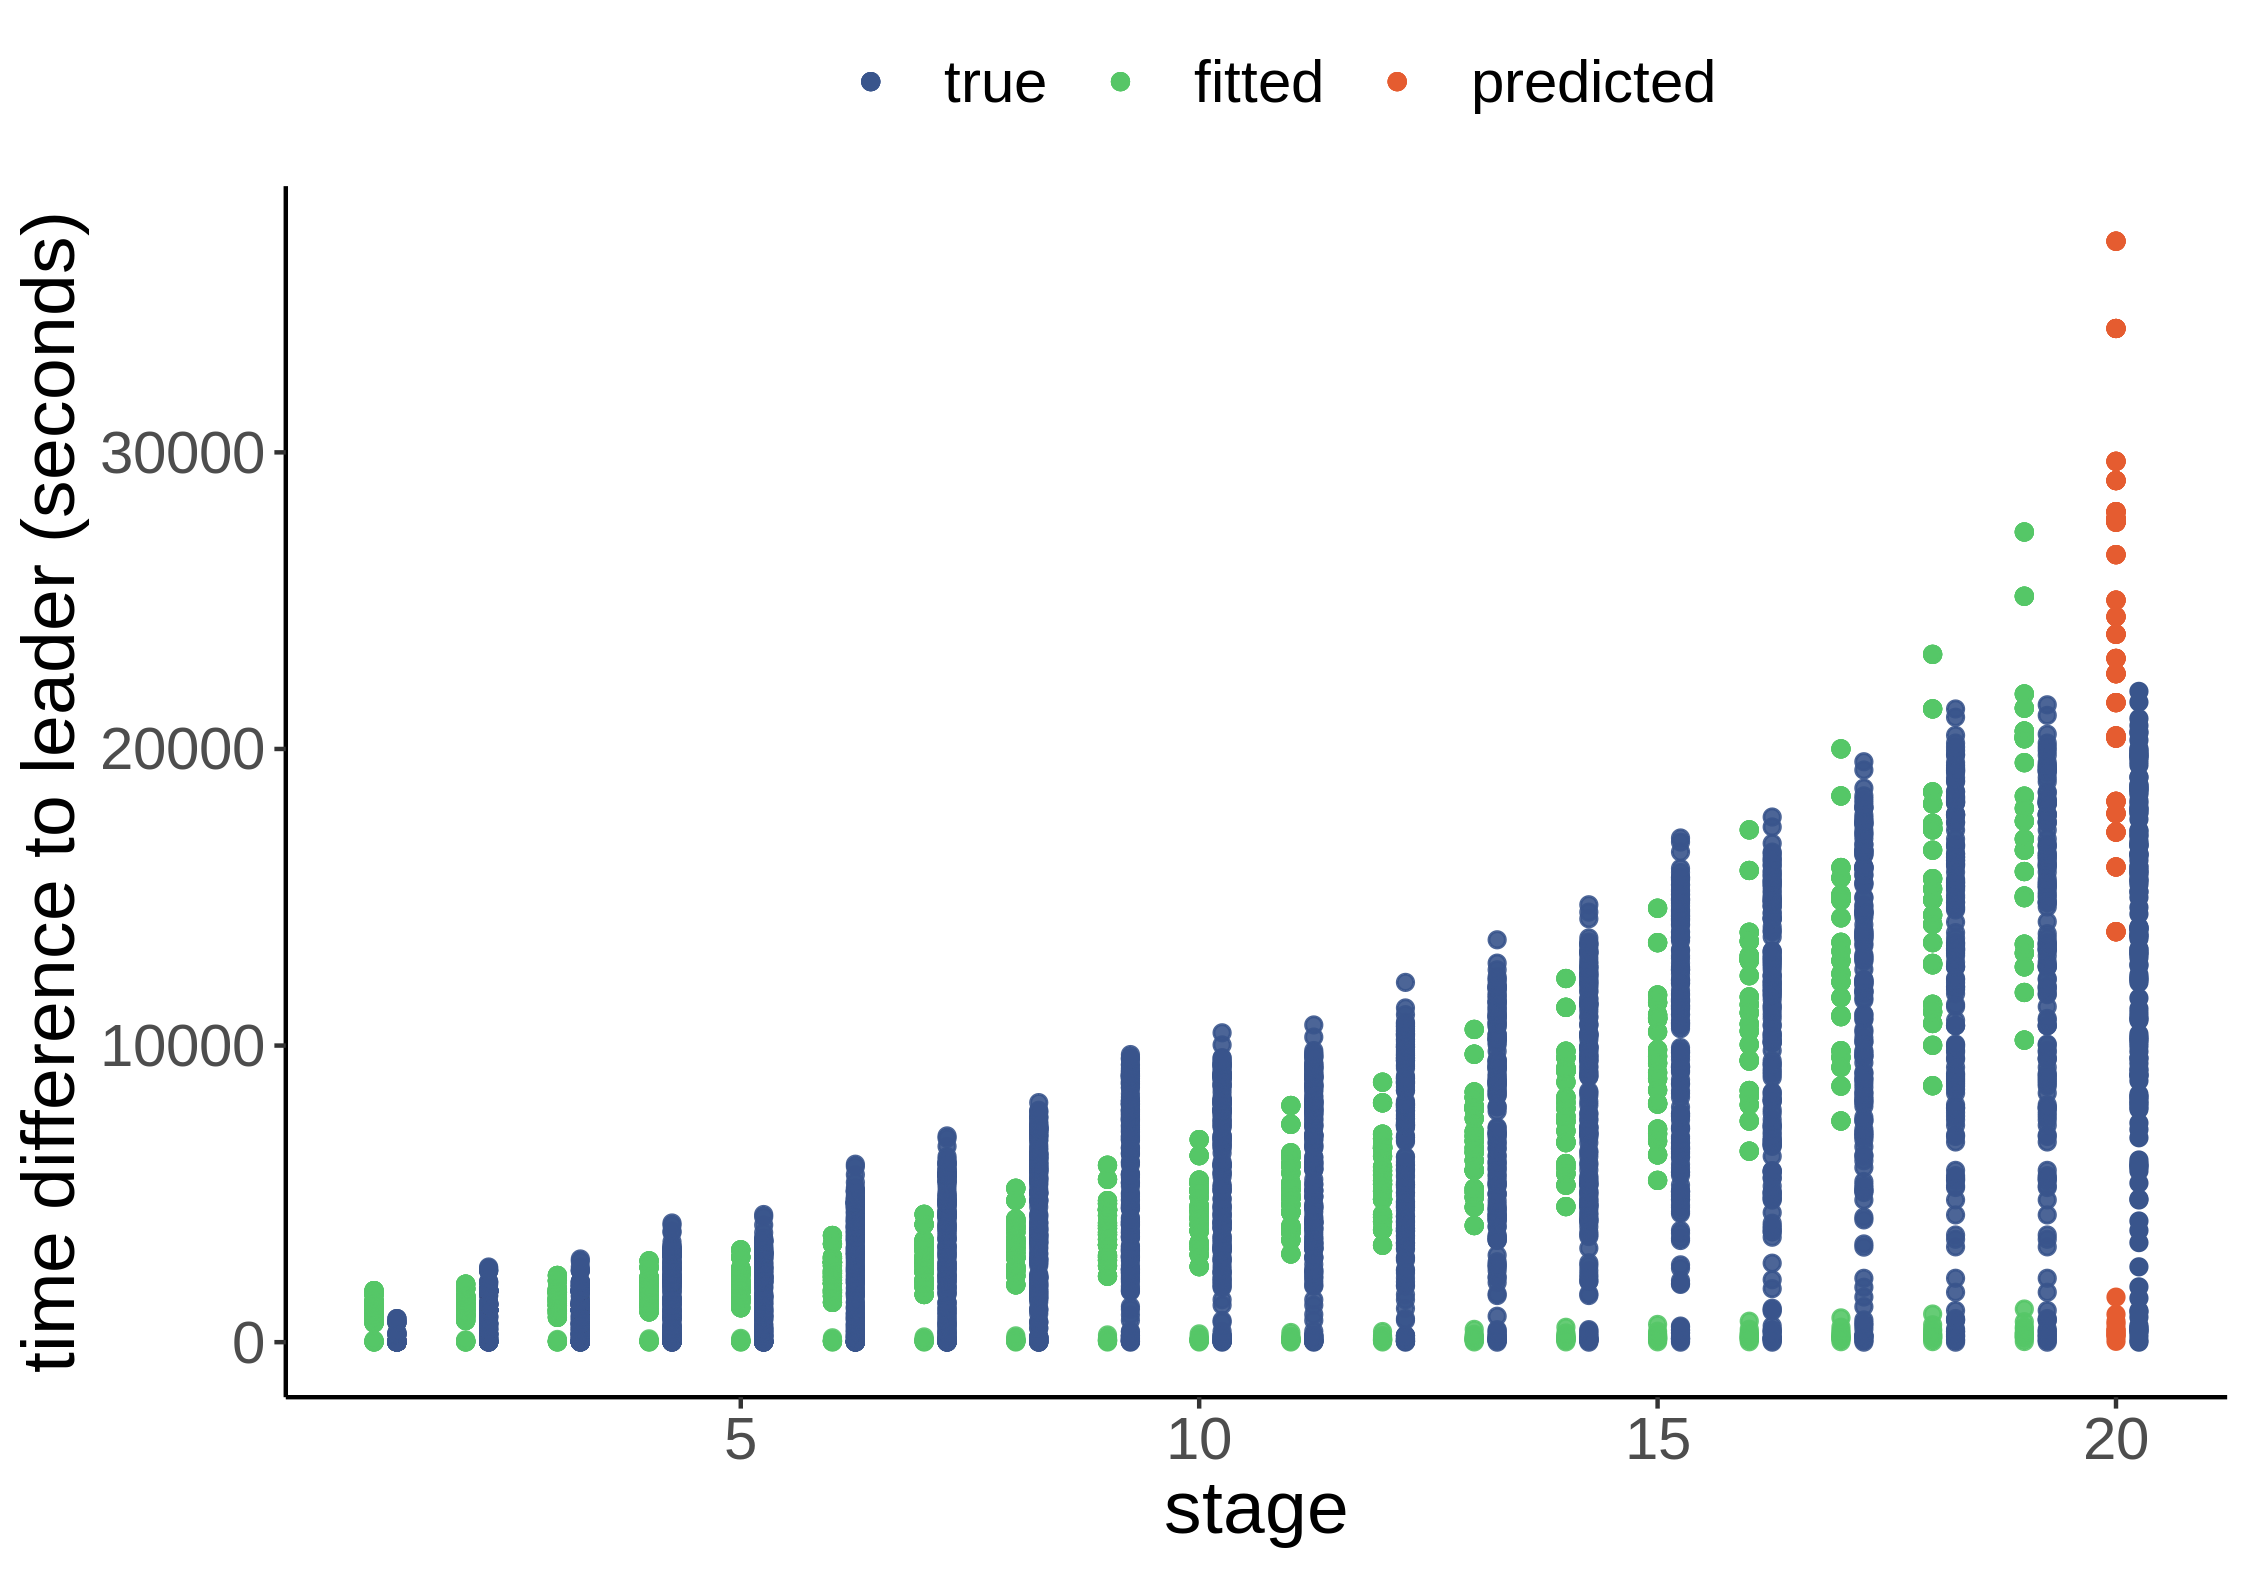
\includegraphics[scale=0.65]{fig/fitted_predicted.png}
  \caption{Comparison of fitted and predicted values against the true values. The compound Poisson-Gamma model successfully captures the increasing variability of observations.}
  \label{fig:fitted_predicted}
\end{figure}


\begin{figure}[h]
  \centering
  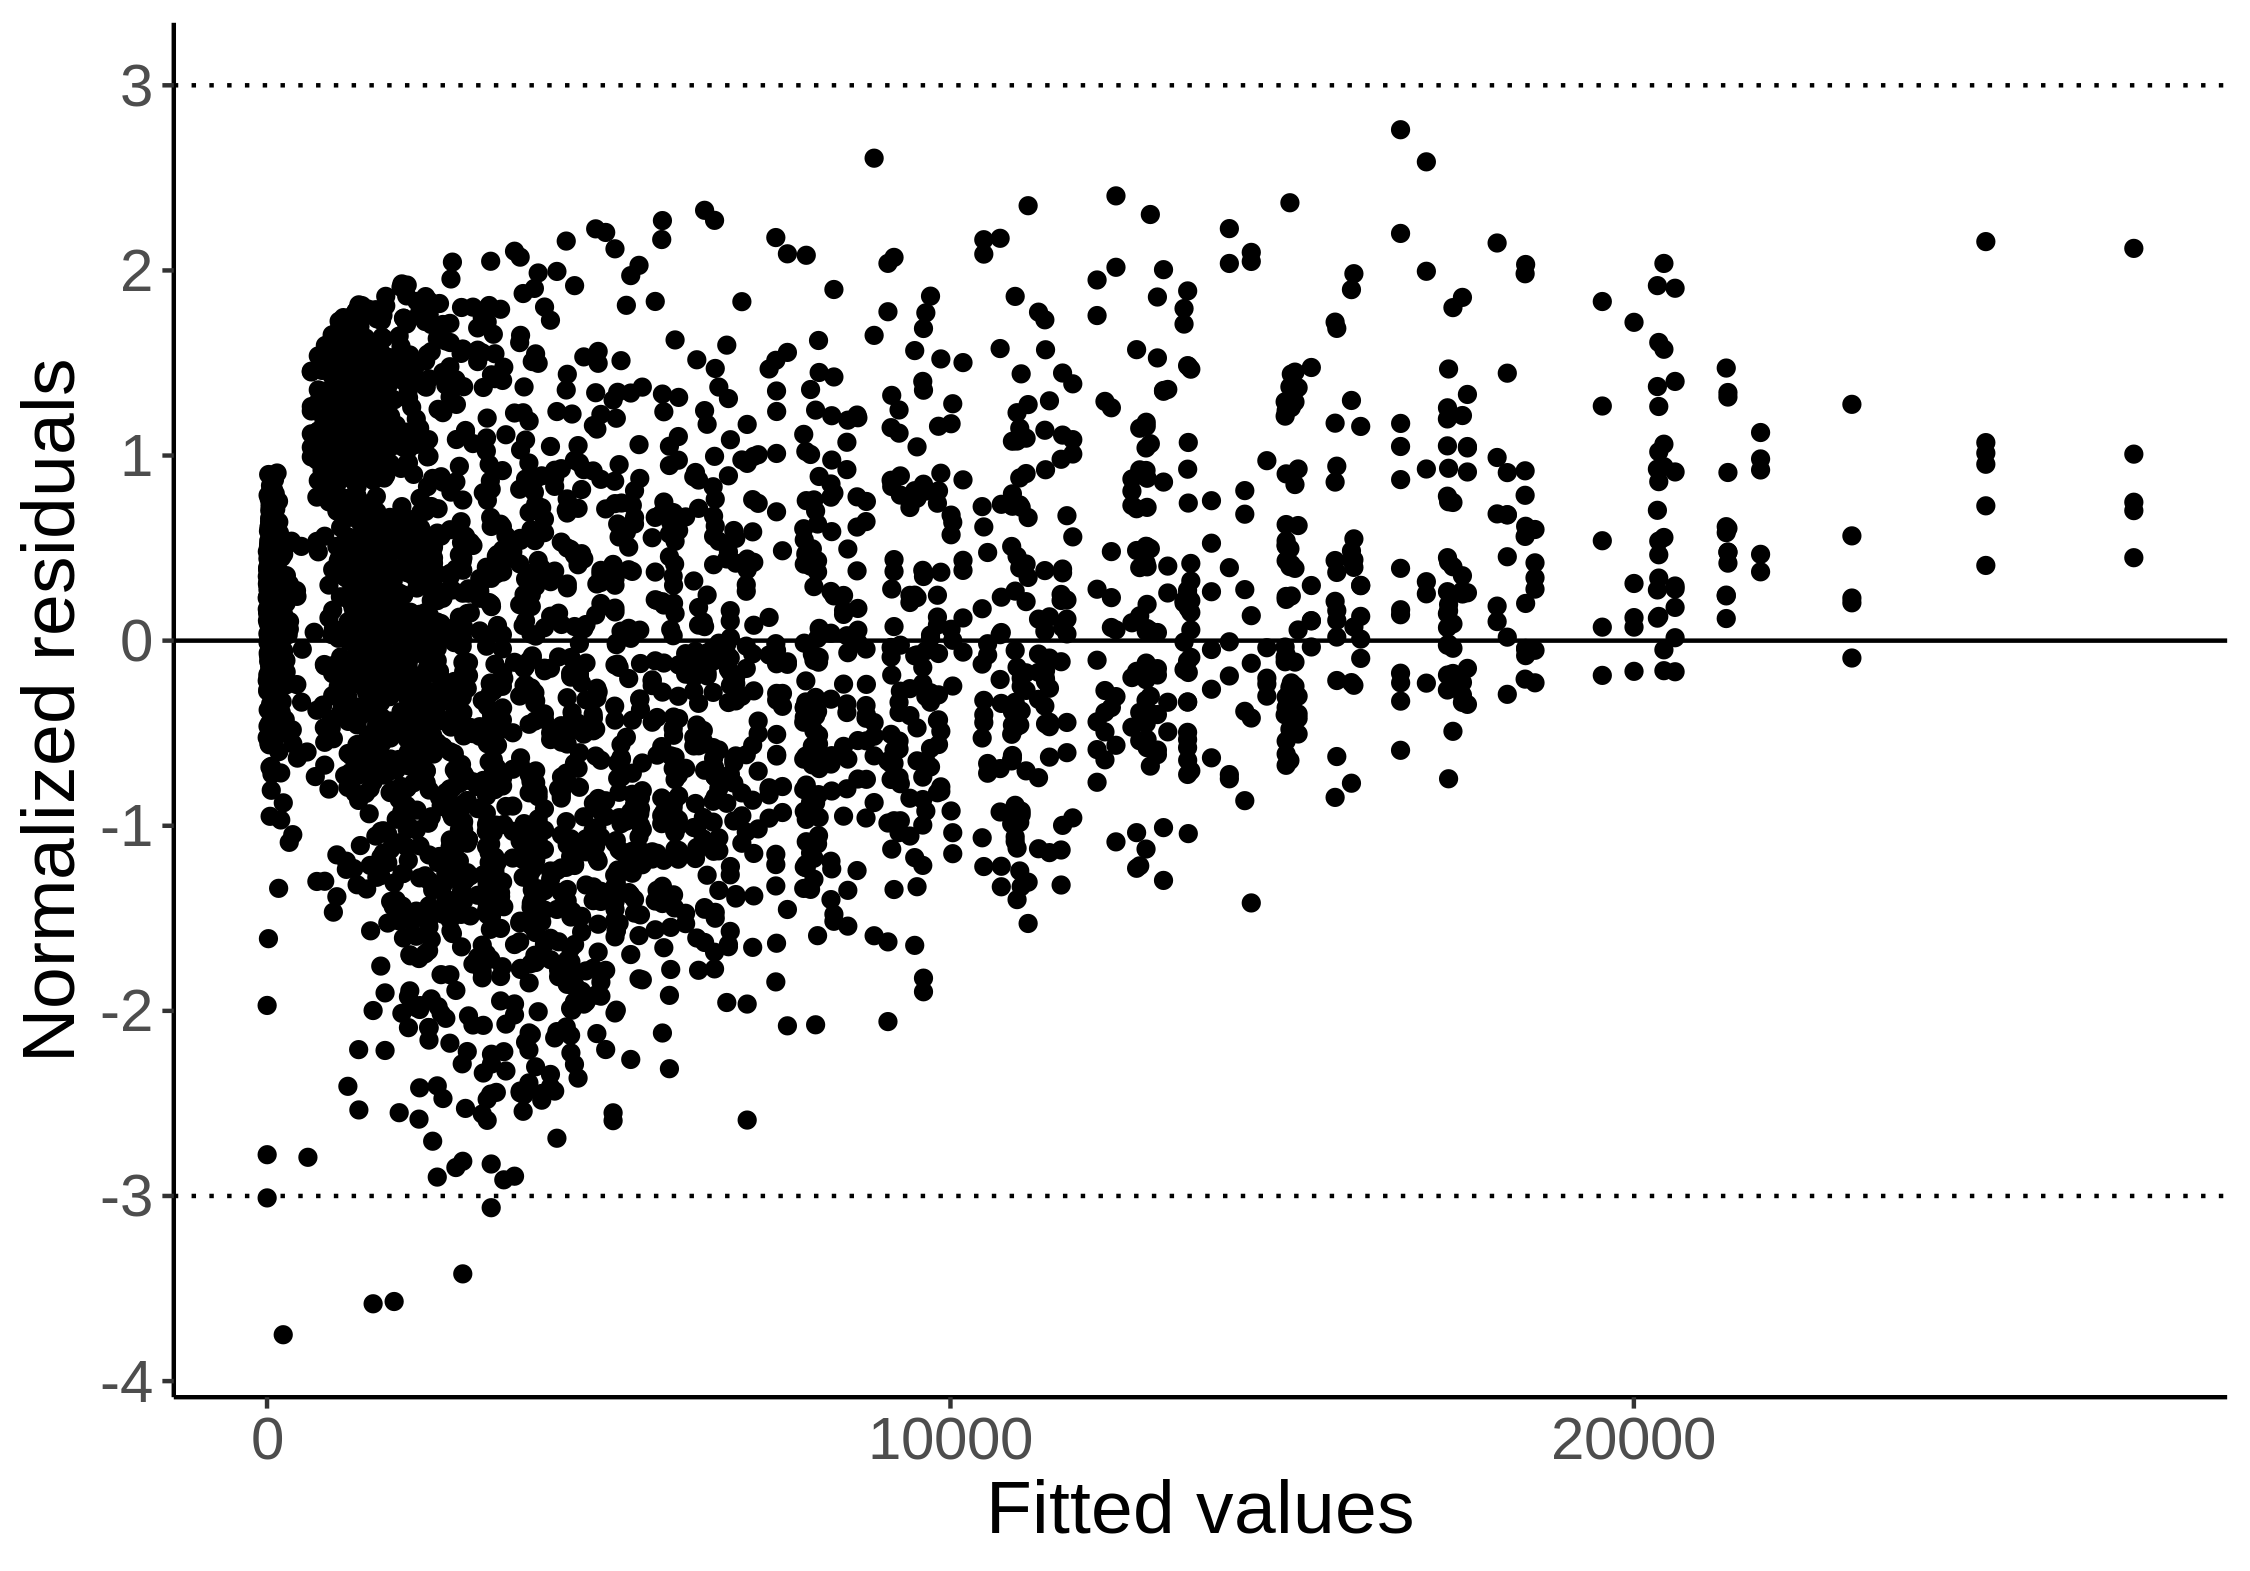
\includegraphics[scale=0.65]{fig/norm_res.png}
  \caption{Normalized residuals of the compound Poisson-Gamma model. The vast majority of values are well within the $\pm$ 3 bound. The model tends to overestimate when fitted values are small and underestimate when they are large.}
  \label{fig:norm_res}
\end{figure}


\begin{table}[ht]
\centering
\begin{tabular}{lccc}
\textbf{Rider}     & \textbf{True ranking} & \textbf{Predicted ranking} & \textbf{\begin{tabular}[c]{@{}c@{}}Predicted probability\\  of winning\end{tabular}} \\ \hline
Tadej Pogačar      & 1                     & 2                          & 0.228                                     \\
Primož Roglič      & 2                     & 1                          & 0.552                                     \\
Richie Porte       & 3                     & 7                          & 0.111                                     \\
Mikel Landa        & 4                     & 6                          & 0.112                                     \\
Enric Mas          & 5                     & 8                          & 0.095                                     \\
Miguel Ángel López & 6                     & 3                          & 0.182                                     \\
Tom Dumoulin       & 7                     & 10                         & 0.052                                     \\
Rigoberto Urán     & 8                     & 4                          & 0.159                                     \\
Adam Yates         & 9                     & 5                          & 0.152                                     \\
Damiano Caruso     & 10                    & 67                         & $<$0.0001                         \\ \hline
\end{tabular}
\caption{Top 10 riders of the 2020 Tour de France. For each rider, its ranking and predicted ranking are shown, along with the predicted probability of winning.}
\label{table:results  }
\end{table}


\section{Conclusion} \label{sec:conclusion}


limitations:
  - cannot model linear relationship between time difference and stage with log link; this is what might cause over and under estimation
  -


\cite{lauderdale2012}


\clearpage
\small
\bibliographystyle{imsart-nameyear}
\bibliography{ref/tdf-2020.bib}

\end{document}
